% 1986 年上海卷理工农医类第 7 题图 2：沿 CP 折成直二面角
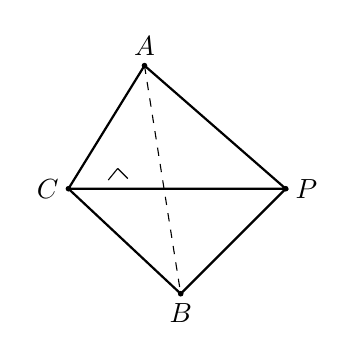
\begin{tikzpicture}[scale=0.92,>=stealth]
  \coordinate (C) at (0,0);
  \coordinate (P) at (3.0,0);
  \coordinate (A) at (1.05,1.7);
  \coordinate (B) at (1.55,-1.45);
  \draw[thick] (C)--(P);
  \draw[thick] (C)--(A)--(P)--cycle;
  \draw[thick] (C)--(B)--(P);
  \draw[dashed] (A)--(B);
  \draw (0.55,0.12)--(0.68,0.28);
  \draw (0.68,0.28)--(0.82,0.14);
  \fill (A) circle (1.1pt) node[above] {$A$};
  \fill (B) circle (1.1pt) node[below] {$B$};
  \fill (C) circle (1.1pt) node[left] {$C$};
  \fill (P) circle (1.1pt) node[right] {$P$};
\end{tikzpicture}
